\section{Results}

% \subsection{Validation Process}

%We need to make sure that our inference algorithm correctly predicts users' income in each of the 5 categories $ H_1, \ldots, H_5 $. According to our hypothesis, the greater the amount of calls to , this increases the probability that both of them will belong to the same group.

%For each link $ p = \left< p_o, p_d, \ldots \right> \in P $, our hypothesis says that $ p_o $ and $ p_d $ will belong to the same income group.

%In order to validate our proposed methodology, we take advantage of the computed $p_lower$ for each user and use this quantity as the predicition score that allow us to evaluate whether a given user belongs to one of the deffined categories. A standarized way to quantify the performace of the metodology is by computing Receiver Operating Characteristic Curve (ROC). This curve

We describe in this section the validation of our methodology.
We examine the true positive ($\TPR$) and false positive ($\FPR$) rates, \( \TPR = \TP / \operatorname{P} \) and \( \FPR = \FP / \operatorname{N} \), where $\TP$ is the number of correctly predicted users with high income, $\operatorname{P}$ is the total number of users with high income, $\FP$ is the number of users incorrectly classified as having high income, and $\operatorname{N}$ is the total number of users with low income.

In Figure~\ref{ROC_multiclass} we plot the ROC (\textit{Receiver Operating Characteristic}) curve, showing $\TPR$ and $\FPR$ for the set of possible values of $\tau$. We see that our methodology clearly outperforms random guessing (dashed straight line). We can summarize our performance by calculating  the $\AUC$ (\textit{Area Under the Curve}) which in Figure~\ref{ROC_multiclass} is $\AUC = 0.74$. Note that random guessing would give a value of $\AUC \simeq 0.50$.


%\vspace{1em}
%
%\begin{adjustwidth}{-1.5cm}{}
%\begin{tabu} to \textwidth { r X[c] X[c] }
%& \multicolumn{2}{ c }{\textbf{Classifier result for income group $ H_i $}} \\
%\\
%& Caller in group & Caller not in group \\
%Callee in group & \cellcolor{green} True Positive & \cellcolor{red} \makecell{False Negative \\ (Type II Error)} \\
%Callee not in group & \cellcolor{red} \makecell{False Positive \\ (Type I Error)} & \cellcolor{green} True Negative \\
%\end{tabu}
%\end{adjustwidth}

%To validate these classifiers, we use

%a \textbf{Receiver Operating Characteristic Curve} (ROC) to plot the \textbf{True Positive Rate} and the \textbf{False Positive Rate} of each system. Since the amount of people in each group is almost equal, randonly guessing each user's income would result in a diagonal line.

%As an objective measurement, we can calculate the \textbf{Area under the curve} for each income group as the chance that the classifier would make a better prediction of the composition of this income group better than a random one. For this we define the density functions $ f_i(x) $ as the probability that a user will be considered part of the income group $ H_i $, and $ g_i(x) $ as the probability that it won't. This way we can characterize the True Positive Rate and the False Positive Rate for each group as

%\vspace{-1em}
%
%\begin{align*}
%\operatorname{TPR}_i(T) &= \int^{\infty}_T f_i(x) dx \\
%\operatorname{FPR}_i(T) &= \int^{\infty}_T g_i(x) dx \\
%\end{align*}
%
%\vspace{-1.5em}

%With this two functions, we can define the AUC for each category as as a simple integration:

%\[
%A_i = P(X_1 > X_0) = \int^{-\infty}_{\infty} \operatorname{TPR_i}(T) \operatorname{FPR_i}(T) dT
%\]

%Where $ X_1 $ is the score for a positive instance, and $ X_0 $ is the score for a negative one.

%\subsection{Results}

\begin{figure}[H]
\begin{center}
{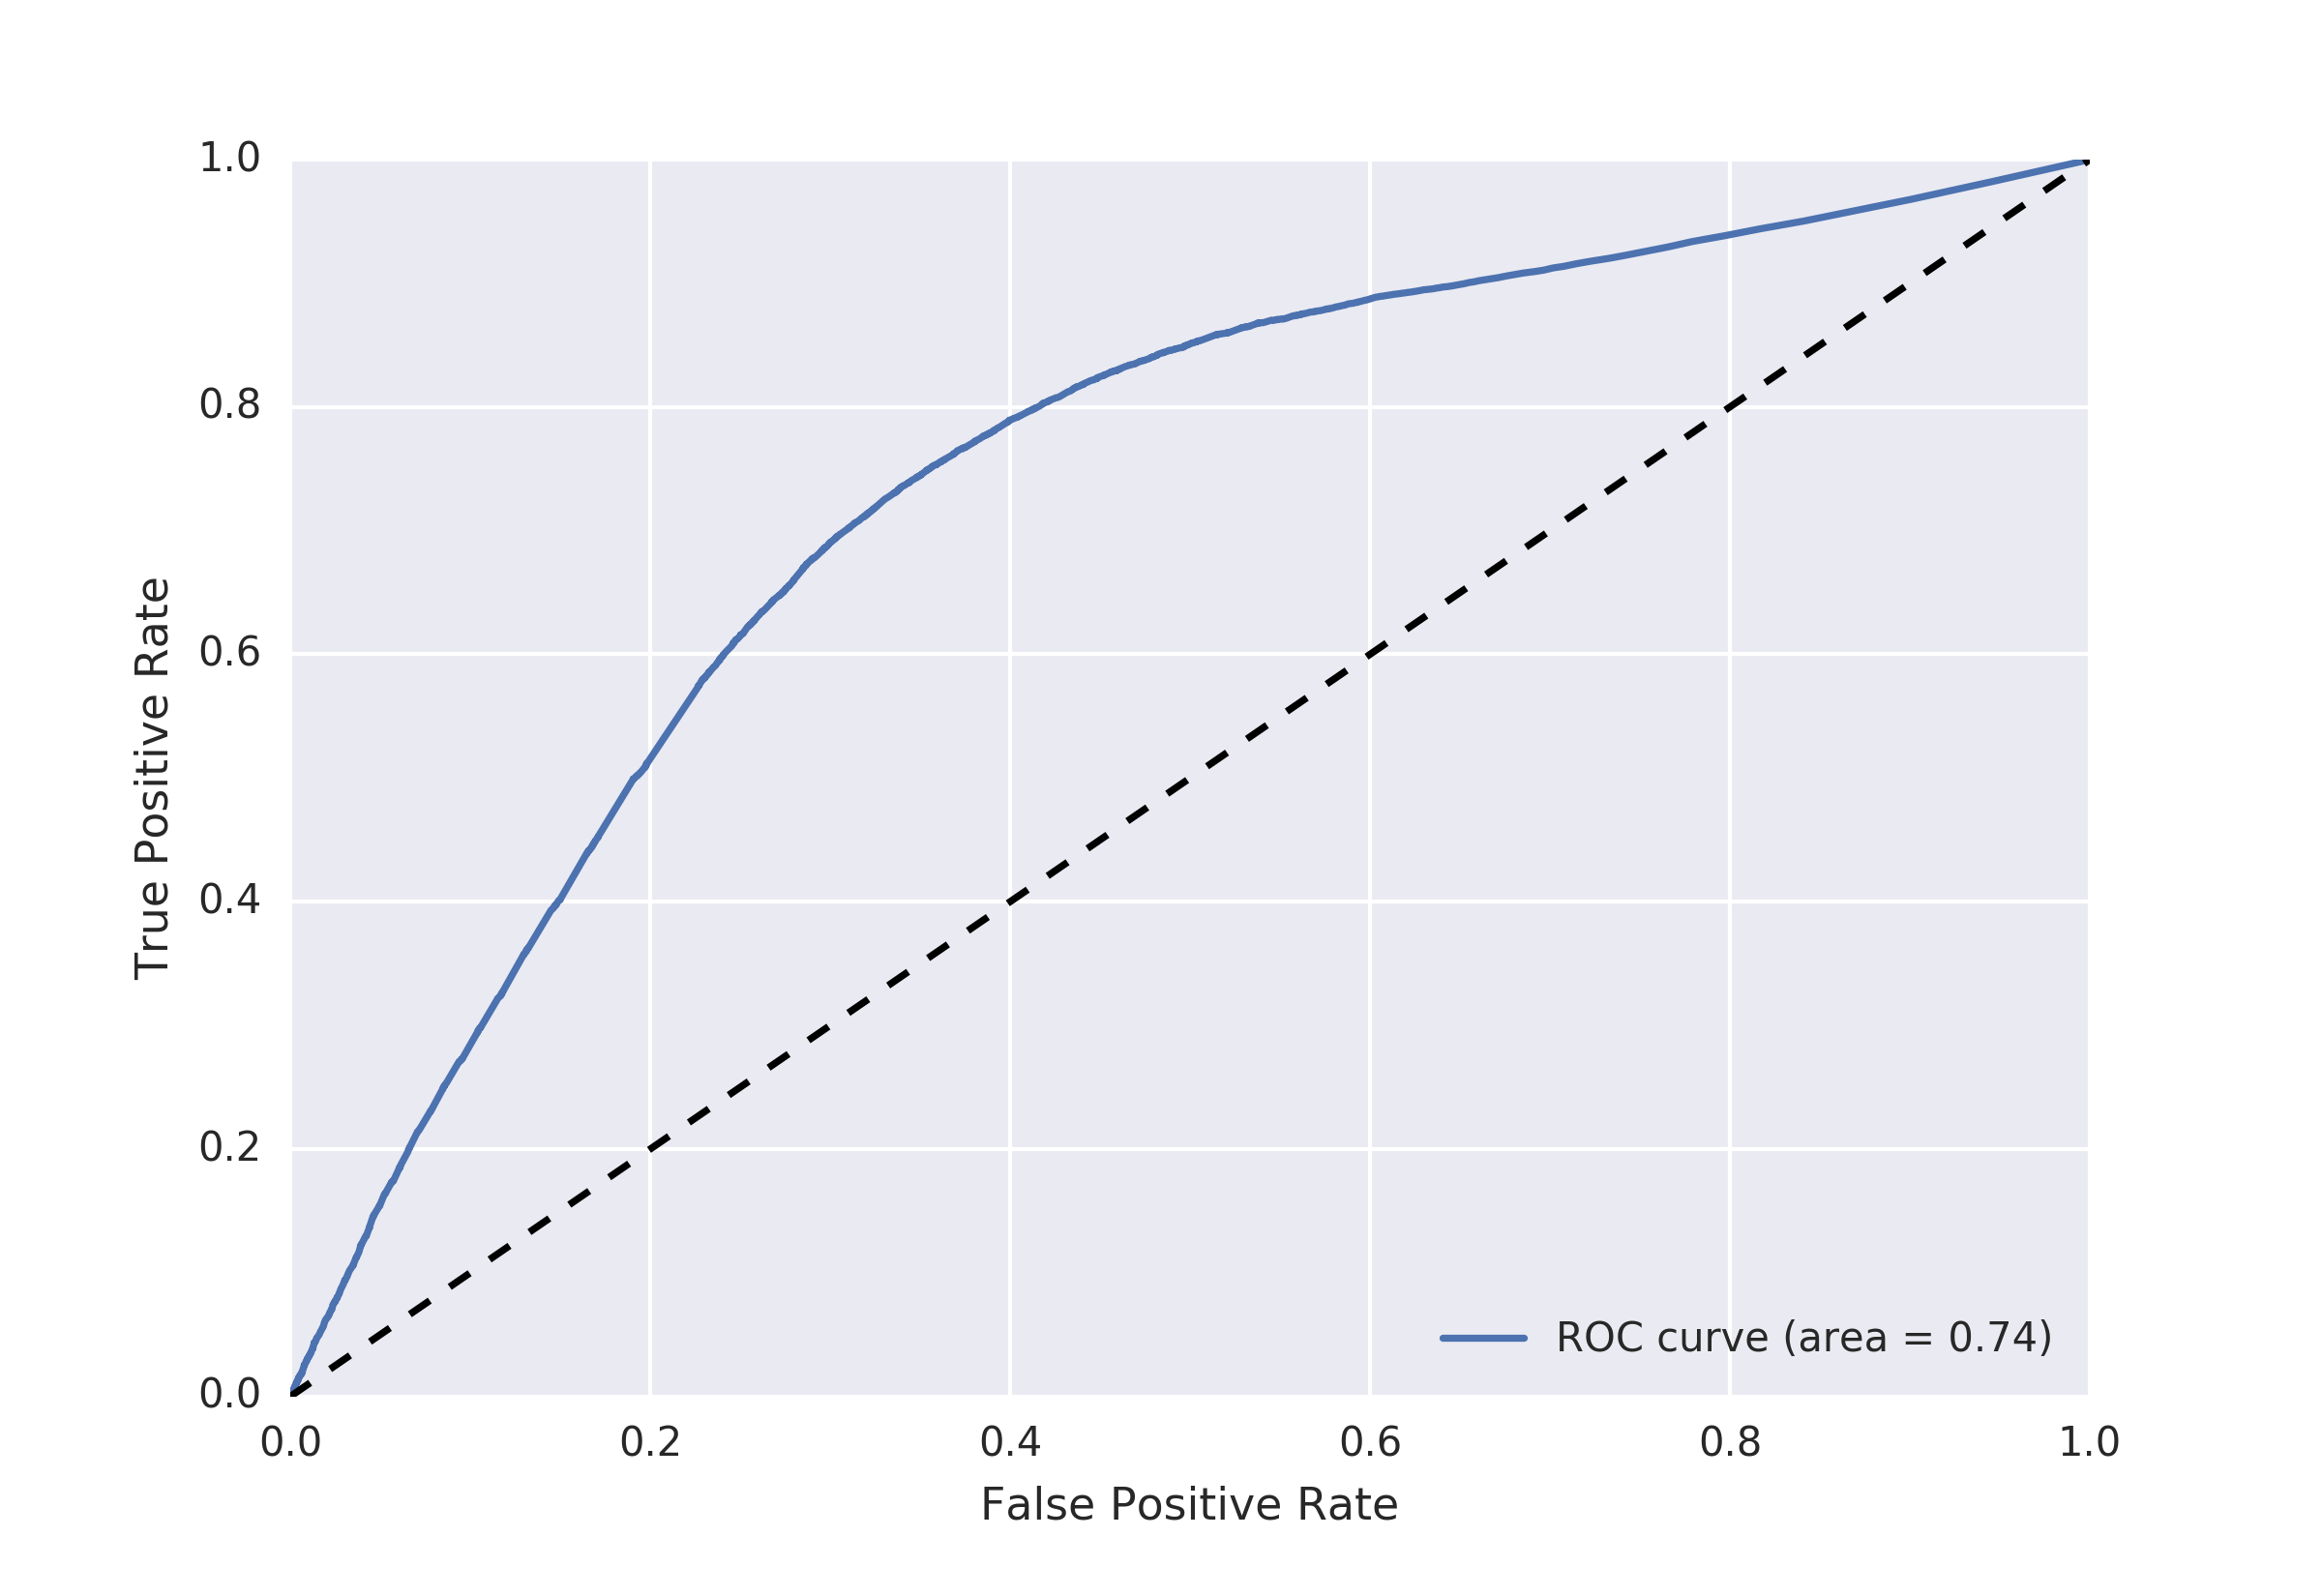
\includegraphics[width=0.85\columnwidth,trim={1.0cm 0.5cm 1.9cm 0.9cm},clip=true]
{figures/ROC_BETA/ROC_Beta_based_approach_201504.png}
}
\caption{ROC curve for prediction procedure. We observed an $\AUC = 0.74$ indicating that our predictor is better than a random predictor ($\AUC \simeq 0.50$).}
\label{ROC_multiclass}
\end{center}
\end{figure}

%We can define the accuracy of the model as the ratio between \(\TP\) and \(\TN\) to total population for a certain \(\FPR\), which gives us values between \num{0.42} and \num{0.71}. The maximum is achieved with an \(\FPR\) of \num{0.4}.

Alternatively we can evaluate the performance of our model by computing its accuracy for a given considered threshold $\tau$. The best accuracy obtained is \num{0.71} for $\tau = 0.4$. 

\subsection{Comparison with other inference methods}

We applied two other inference methods to the same data and compared their accuracies to our Bayesian model.

\begin{itemize}
	\item \textbf{Random selection} which chooses randomly the category for each user.
	\item \textbf{Majority voting} which decides whether a user is in the high or low income category depending on the category of the majority of its contacts. In case of a tie, the category is chosen randomly.
\end{itemize}

The accuracy of the first method is as expected \num{0.50}, while the accuracy for majority voting is \num{0.66}. 
With the Bayesian method we obtain an accuracy of \num{0.71}.
